\chapter{Project plan}
\label{cha:plan}

The plan for this project more or less follows on from the evaluation of the precious one~\cite{gillian-debugging-2021}.

\section{Improving the debuggomg experience}

\subsection{Building a custom debugging UI}

As stated in \autoref{sec:intro:debugging}, the DAP doesn't have the command
set necessary for debugging symbolic exectuion. We can, however, use a
combination of Webviews and custom DAP requests / events to supplement the
existing debugging UI (see \autoref{sec:background:extending-dap}).

\subsection{Selecting symbolic execution branches}

A prime missing feature as the debugger stands is the ability for users to select branches of execution when debugging. Currently, the debugger runs through the problem top-to-bottom, dealing with each branch in turn. Ideally, users will able to select which branch to go down when given a choice.

\begin{figure}
  \noindent
  \makebox[\textwidth]{
    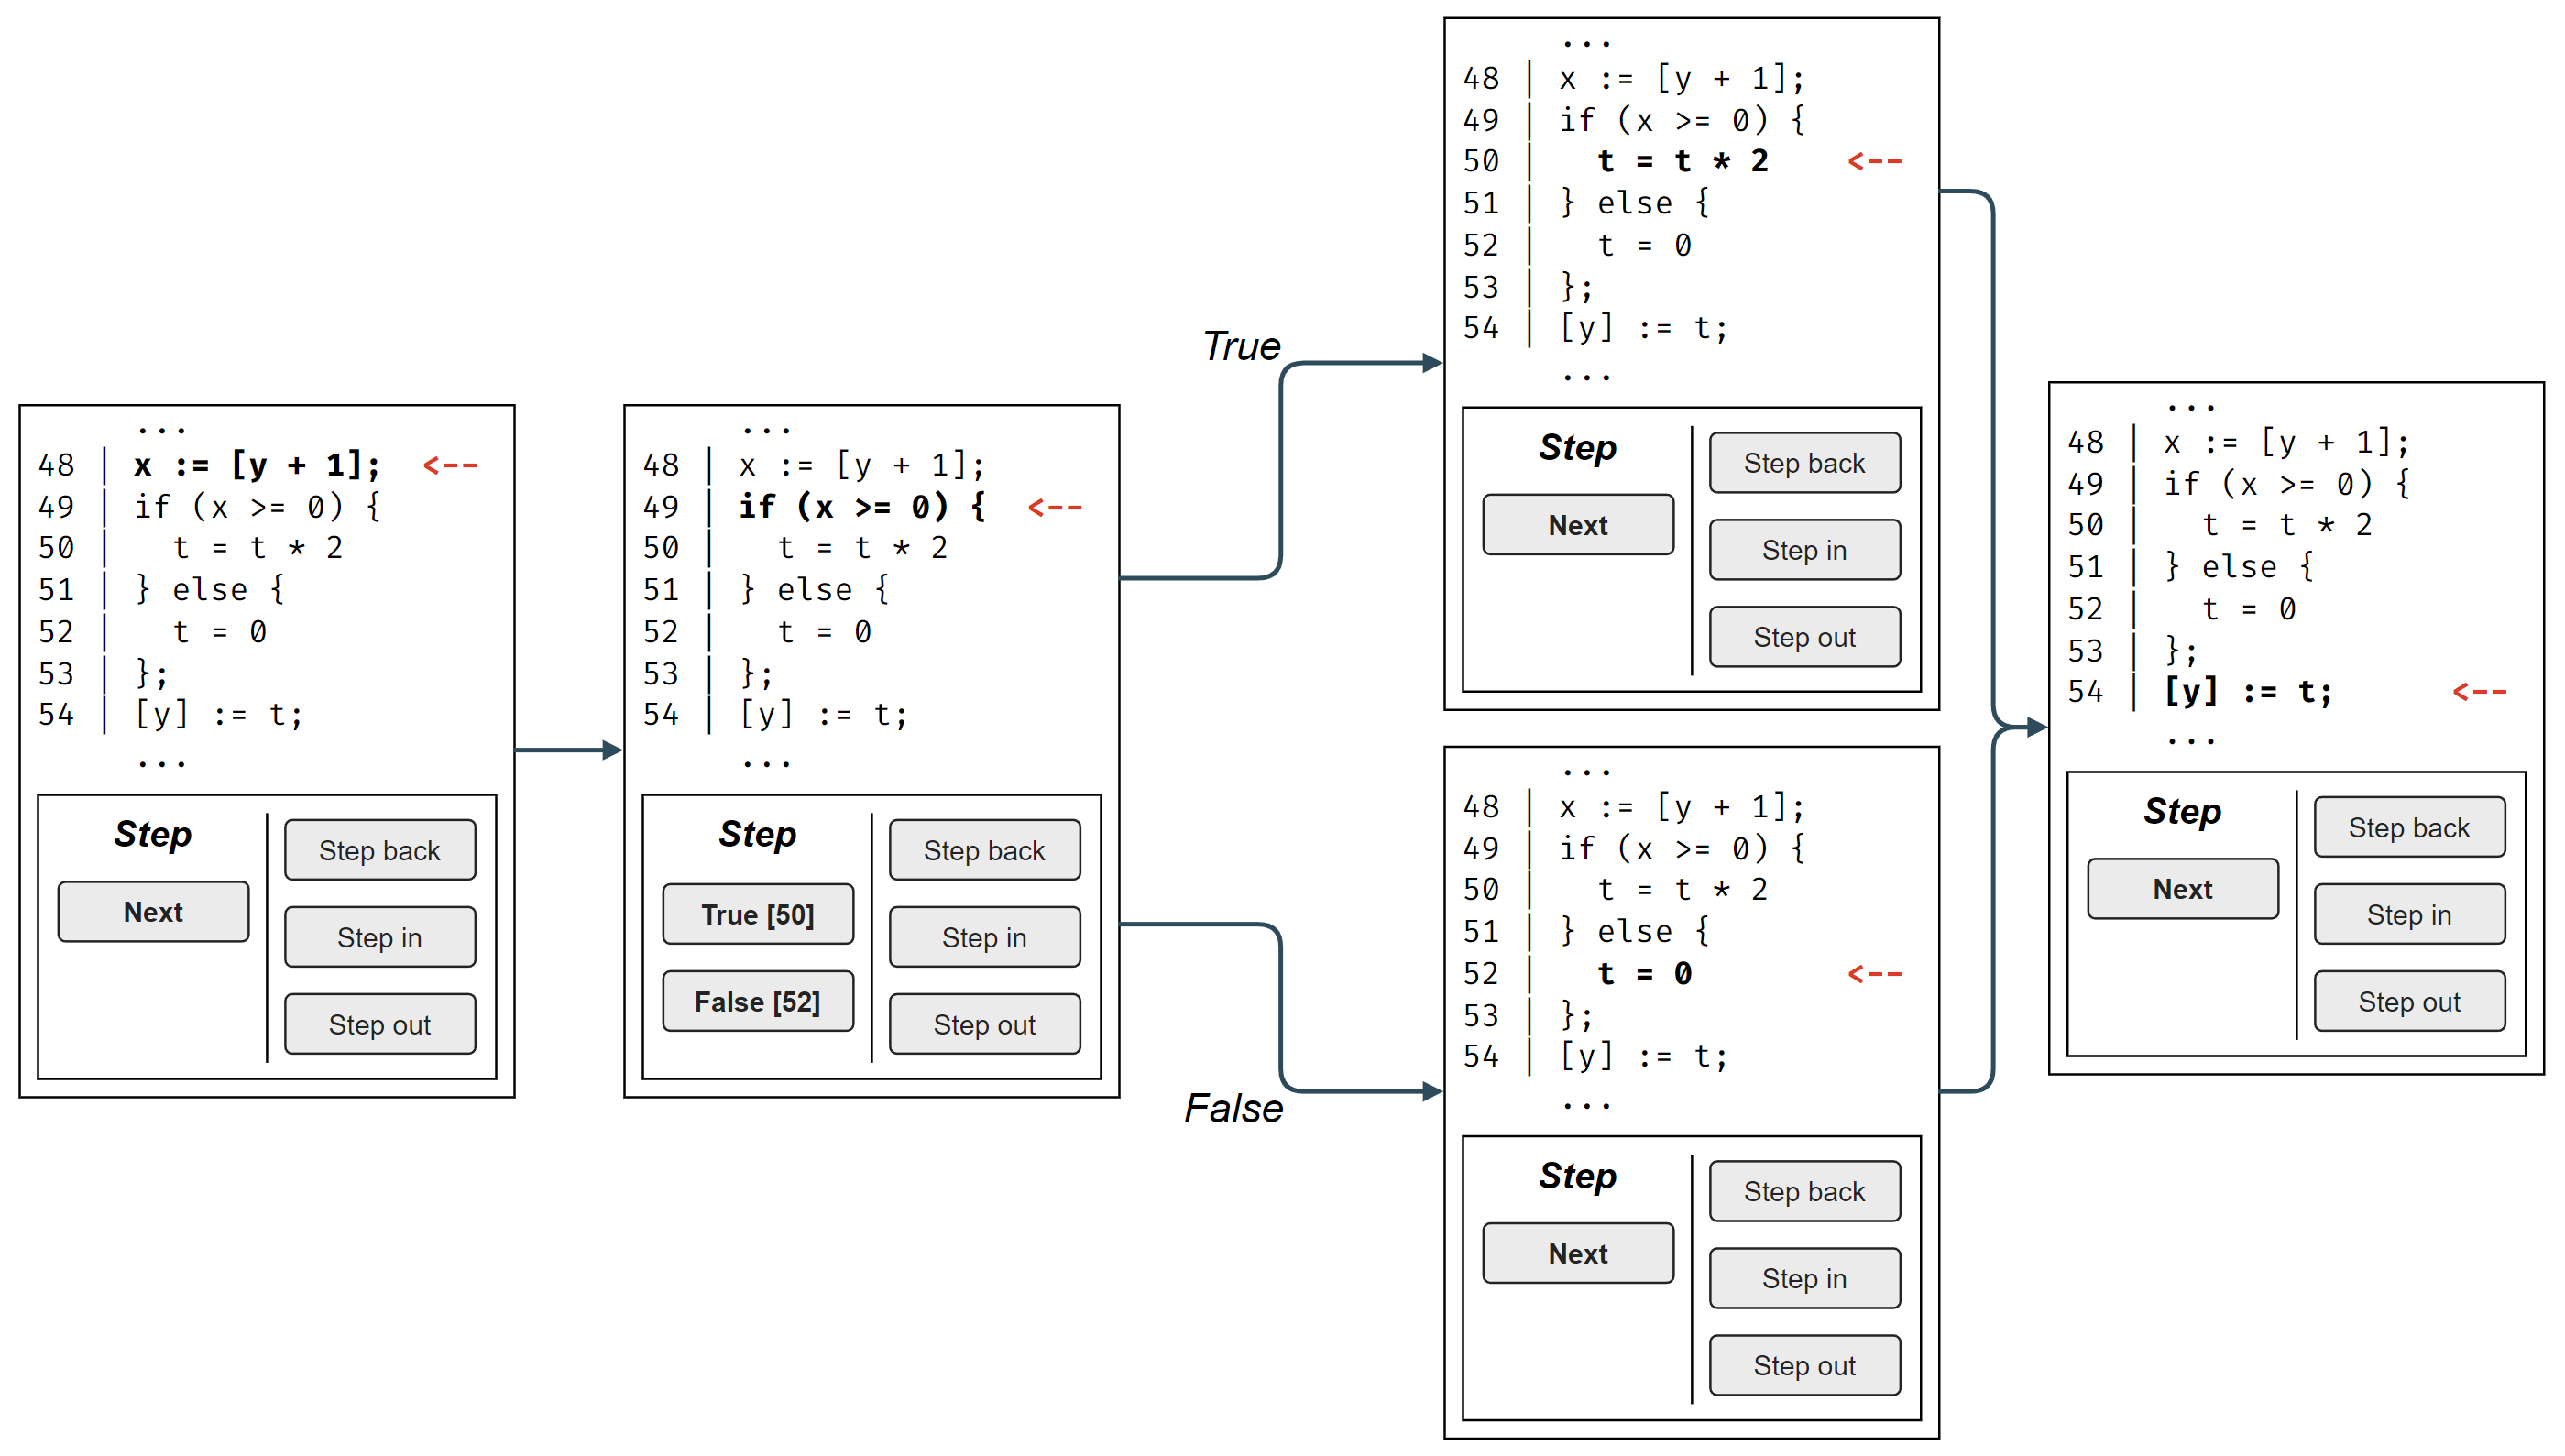
\includegraphics[width=500px]{img/branch-selection-mockup.png}
  }
  \caption{A mockup of a potential UI flow for selecting execution branch.}
  \label{fig:branch-selection-mockup}
\end{figure}

As a bare minimum, this should be implemented for if-else statements; ideally,
this should be extened to cover switch statements, as well as any other
branching statements in the target languages supported.

% Maybe run an HTTP server when debugging to serve the extra info and controls?

\subsection{Improving error message coverage}

\subsection{Miscellaneous quality-of-life features}

\section{Gillian-Rust}
% What am I doing with Rust? Just implementing a debugger component for it?
